%------------------------------------------------------------------------------
% Author(s):
% Brad Bachu, Varaun Ramgoolie
%
% Copyright:
%  Copyright (C) 2020 Brad Bachu, Arjun Mohammed, Varaun Ramgoolie, Nicholas Sammy
%
%  This file is part of Applied-Mathematics-Unit2 and is distributed under the
%  terms of the MIT License. See the LICENSE file for details.
%
%  Description:
%     Year: 2014
%     Module: 3
%     Question: 5*
%------------------------------------------------------------------------------

%------------------------------------------------------------------------------
% 5 a
%------------------------------------------------------------------------------
	
\begin{subquestions}
	
	\subquestion
	
	We are given the displacement function of a particle, from a fixed point $O$, as it moves along a straight line.
	
	\begin{subsubquestions}
		
		\subsubquestion
		
		\rfig{2014:q5*:SGraph1} shows the displacement-time graph of the particle.
		\begin{figure}[H]
			\begin{center}
				\includegraphics{../2014/figures/DispGraph-2014-q5-a-i}
				\caption{\label{2014:q5*:SGraph1} Displacement-time graph of the particle's motion.}
			\end{center}
		\end{figure}
		
		It is useful to interpret the different regions of this graph so that we can get a stronger understanding of the motion of the particle. Using the given $s(t)$, we can see that the roots of the graph (points at which $s=0$) must occur when $t=2$ and $t=6$. We can also notice that the graph is a `U' shape as the graph of $s(t)$ is quadratic with a positive $t^2$ coefficient. 
		
		For $0 \leq t < 2$, we can see that the displacement of the particle is positive, from the fixed point $O$. For $2 < t < 6$, the displacement is negative and for $t>6$, the particle's displacement is positive. 
		
		We know that the gradient of a displacement-time graph is equivalent to velocity of the particle at any point in time. Therefore, we can notice that the velocity of the particle is negative for $12 \leq t < 4$ and positive for $t>4$ (this is indicative of the particle moving in the negative direction for $0 \leq t < 4$ and in a positive direction for $t>4$). 
		
		At $t=4$, we see that the motion of the particle seems to `turn around' and the velocity changes from negative to positive. 
		
		%------------------------------------------------------------------------------
		
		\subsubquestion
		
		\begin{subsubsubquestions}
			
			\subsubsubquestion
			
			\textbf{\textit{Simplify and Diagram:}} \\ \\
			
			\begin{figure}[H]
				\begin{center}
					\includegraphics{../2014/figures/DispGraph2-2014-q5-a-ii}
					\caption{\label{2014:q5*:SGraph2} Displacement-time graph of particle.}
				\end{center}
			\end{figure}
			
			We want to find the distance traveled from $t=0$ to $t=5$ (green line in \rfig{2014:q5*:SGraph2}). From \rfig{2014:q5*:SGraph1}, we know that the graph changes direction at $t_m=4$. This means that, in order to find the total distance traveled, we have to consider two pieces of the graph separately and sum their results. We do this because, in the period of time given, the particle moves in opposite directions (which increases the change in distance but decreases the change in displacement). We will consider $0 \leq t < 4$ and $4 < t < 5$ separately.
			
			By definition, if we integrate the velocity of the particle, we will get the displacement of the particle between the bound of integration. If we instead integrate the \textbf{modulus} of the velocity, we will get the distance traveled by the particle.\footnote{By integrating the modulus of the velocity, we consider the particle's movement as solely 'positive'. Therefore, the integral of this modulus function will sum only 'positive' displacements. The sum of these 'positive displacements will therefore give us our total distance traveled.}
			
			
			
			\textbf{\textit{Represent Mathematically:}} \\ \\
			To obtain our distance traveled, we will integrate our velocity function. By definition, we get that,
			\begin{align}
				v(t) & = \ddd{}{t}s(t) \nn \\ 
				     & = \ddd{}{t}(t^2-8t+12) \nn \\
				     & = 2t-8 \,.
			\end{align}
			
			It is helpful to examine this function (and its modulus) graphically. See \rfig{2014:q5*:VGraph1}.\footnote{If we only integrate $v(t)$, we will get a negative sum for the integral between $t=0$ and $t=4$. The modulus sign ensures that all of our integration results in positive values.}
			\begin{figure}[H]
				\begin{center}
					\includegraphics{../2014/figures/VeloctyGraph-2014-q55}
					\caption{\label{2014:q5*:VGraph1} Velocity-time graph of the particle}
				\end{center}
			\end{figure}
		
			To find the distance from $t=0$ and $t=5$, we can integrate $|v|=|2t-8|$ between these bounds as follows,
			\begin{align}
				\text{Distance} & = \int_{0}^{5} (|v|)\dd t \nn \\
				                & = \int_{0}^{5} (|2t-8|)\dd t \nn \\
				                & = \int_{0}^{4} (|2t-8|)\dd t  + \int_{4}^{5} (|2t-8|)\dd t \nn \\
				                & = -\int_{0}^{4} (2t-8)\dd t  + \int_{4}^{5} (2t-8)\dd t \,. 
			\end{align}\footnote{The negative sign in the first integral reverses the sign of the result so that it is a positive value.}
						
			\textbf{\textit{Solve and Evaluate:}} \\ \\
			Evaluating our integral, we get that,
			\begin{align}
				\text{Distance} & = -\int_{0}^{4} (2t-8)\dd t  + \int_{4}^{5} (2t-8)\dd t \nn \\
				                & = -\left[t^2-8t \right]_0^4 + \left[t^2-8t \right]_4^5 \nn \\
				                & = -\left[(4^2-32)-(0^2-0)\right] + \left[(5^2-40)-(4^2-32)\right] \nn \\
				                & = -(-16-0) + (-15 - (-16)) \nn \\
				                & = 16+1 \nn \\
				                & = 17 \text{m} \,. 
			\end{align}
			
			%------------------------------------------------------------------------------
			
			\subsubsubquestion
			
			\textbf{\textit{Simplify and Diagram:}} \\ \\
			We want to find the average velocity over $t=0$ to $t=5$. In this case, we need to find the displacement over this period. Then, in order to find the average velocity, we divide that displacement by the time taken (as per the definition of average velocity). \\
			
			
			
			\textbf{\textit{Represent Mathematically:}} \\ \\
			To find the displacement from $t=0$ to $t=5$, we do not have to consider any changing directions. We can directly find the displacement using,
			\begin{align}
				s_{t=0 \rightarrow 5} & = \text{Final Displacement - Initial Displacement} \nn \\
				& =  s(5)-s(0) \,. \label{2014:q5*:Seqn4} 
			\end{align}
			
			Using the definition of average velocity, we can find that,
			\begin{align}
				v_{avg(t=0 \rightarrow 5)} & = \frac{s_{t=0 \rightarrow 5}}{\Delta t} \nn \\
				& = \frac{s_{t=0 \rightarrow 5}}{5-0} \,. \label{2014:q5*:Seqn5}
			\end{align}
			
			
			
			\textbf{\textit{Solve and Evaluate:}} \\ \\
			Using \req{2014:q5*:Seqn4}, we can find,
			\begin{align}
				s_{t=0 \rightarrow 5} & =  s(5)-s(0) \nn \\
				& = -3 - 12 \nn \\
				& = -15 \text{m} \,.
			\end{align}
			
			Using \req{2014:q5*:Seqn5}, we get that,
			\begin{align}
				v_{avg(t=0 \rightarrow 5)} & =\frac{s_{t=0 \rightarrow 5}}{5-0} \nn \\
				& = \frac{-15}{5-0} \nn \\
				& = -3 \text{ms}^{-1} 
			\end{align}
			
			%------------------------------------------------------------------------------
			
			\subsubsubquestion
			
			\textbf{\textit{Simplify and Diagram:}} \\ \\
			We are given that the displacement of the particle, $s(t)$, is a function of time. By definition, we know that the velocity of the particle, $v(t)=\frac{d}{dt}(s(t))$. Therefore, we can find the derivative of $s(t)$ and find the value of $t$ which makes that derivative 0.
			
			
			
			\textbf{\textit{Represent Mathematically:}} \\ \\
			By definition, we get that,
			\begin{equation}
				v(t) = \ddd{}{t}(s(t)) \,. 
			\end{equation}
		
		
		
			\textbf{\textit{Solve and Evaluate:}} \\ \\
			By differentiating $s(t)$, we get that,
			\begin{align}
				v(t) & = \ddd{}{t}(s(t)) \nn \\
				     & = \ddd{}{t}(t^2-8t+12) \nn \\
				     & = 2t-8 \,.
			\end{align}
			
			We can now set $v(t)$ equal to 0 and find the corresponding value of $t$.
			\begin{align}
				v(t) = 2t-8 & = 0 \nn \\
				       2t & = 8 \nn \\
				       \implies t & = 4\text{s} \,.
			\end{align}
			
			Thus, we get that, at $t=4$, the velocity of the particle is 0 (stationary). \\
			
			In addition to this, another intuition that can motivate this solution is that the quadratic of $s(t)$ must be symmetric about its minimum point. As we have already discussed in the first solution, we know that this minimum point must be the point where the velocity is 0. From $s(t)=(t-2)(t-6)$, we can see that the roots are $t=2$ and $t=6$. Therefore, the minimum point must occur at the midpoint of these roots which means that the midpoint occurs at $t=\frac{2+6}{2}=4$.
		\end{subsubsubquestions}
		
	\end{subsubquestions}

%------------------------------------------------------------------------------
% 5 b
%------------------------------------------------------------------------------
 
\subquestion

\begin{subsubquestions}
	
	\subsubquestion
	
	\textbf{\textit{Sketch and Translate:}} \\ \\
	We are given a series of forces which act on a particle with mass, $m$. \rfig{2014:q5:Force1} shows all the forces acting on the particle.
	\begin{figure} [H]
		\begin{center} 
			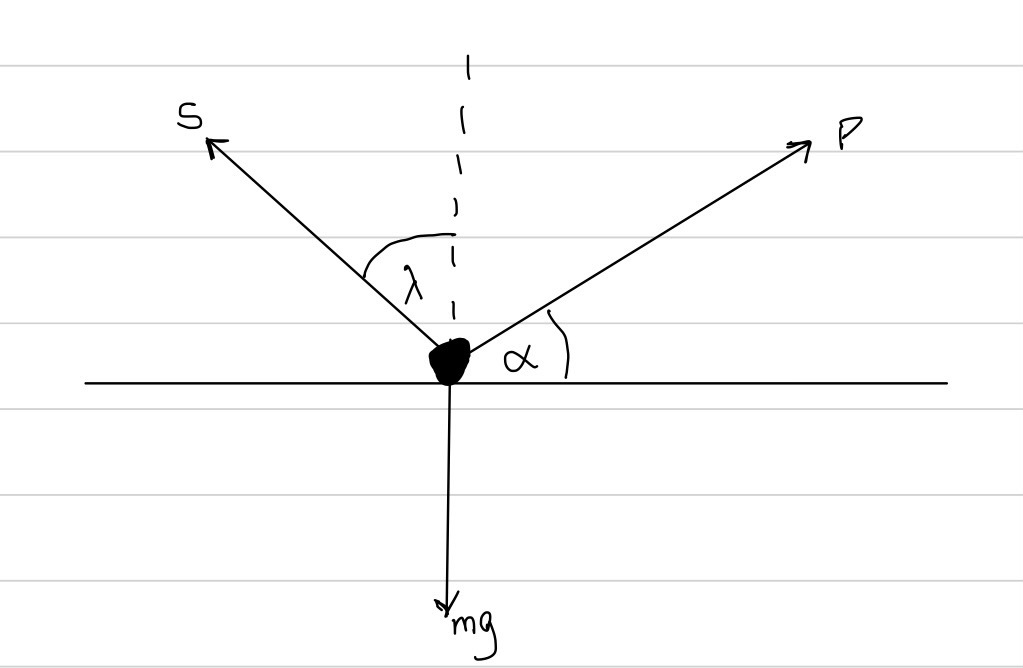
\includegraphics[scale=0.25]{../2014/figures/2014-q5-b-1}
			\caption{\label{2014:q5:Force1} Diagram of forces on particle.}
		\end{center}
	\end{figure}
	
	%------------------------------------------------------------------------------
	
	\subsubquestion
	
	\textbf{\textit{Simplify and Diagram:}} \\ \\
	\rfig{2014:q5:Force2} shows all the forces acting on the particle.
	\begin{figure} [H]
		\begin{center} 
			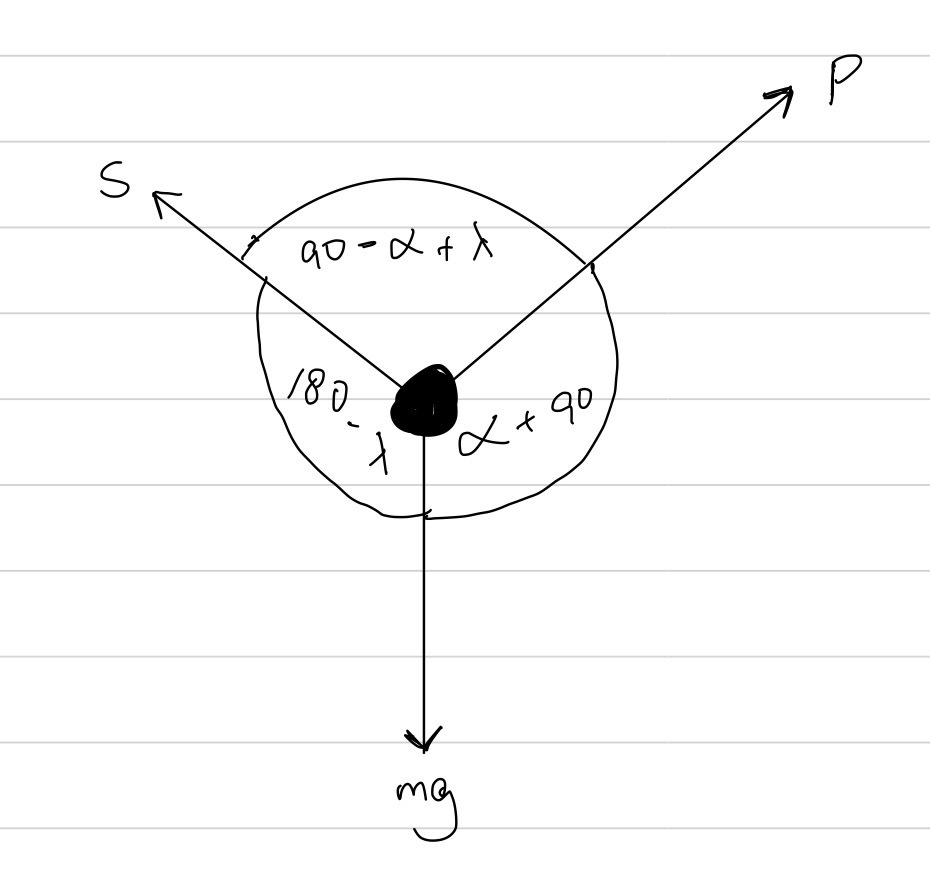
\includegraphics[scale=0.25]{../2014/figures/2014-q5-b-2}
			\caption{\label{2014:q5:Force2} Diagram of forces and angles on particle.}
		\end{center}
	\end{figure}
	
	We are given that the size of $P$ is such that the particle is just about to move. To find the least value of $P$, we need to find a closed form expression of $P$ and minimize it. As the particle has 3 forces acting on it, we can use Lami's theorem to isolate an expression for $P$.
	
	\textbf{\textit{Represent Mathematically:}} \\ \\
	Using Lami's theorem on the particle, we get,
	\begin{equation}
		\frac{mg}{\sin(90-\alpha+\lambda)} = \frac{P}{\sin(180-\lambda)} = \frac{S}{\sin(\alpha+90)} \,.
	\end{equation}
	
	We can consider the $mg$ and $P$ terms and make $P$ the subject of the formula. Doing this, we get,
	\begin{align}
		\frac{P}{\sin(180-\lambda)} & = \frac{mg}{\sin(90-\alpha+\lambda)}\nn \\
		P & = \frac{mg\sin(180-\lambda)}{\sin(90-(\alpha-\lambda))}\,.
	\end{align}
	
	Since we know that $\sin(90-k)=\cos(k)$, we can express $P$ as,
	\begin{align}
		P & = \frac{mg\sin(180-\lambda)}{\sin(90-(\alpha-\lambda))} \nn \\
		& = \frac{mg\sin(180-\lambda)}{\cos(\alpha-\lambda)} \,.
	\end{align}
	
	\textbf{\textit{Solve and Evaluate:}} \\ \\
	As we have a closed form for $P$, we can work to minimize this expression. We should notice that $P$ has a denominator of $\cos(\alpha - \lambda)$. This means that, in order to minimize $P$, we have to maximize this denominator. The Cosine function has a maximum value of 1 and this occurs when the argument of the function is equal to 0. This implies that the argument of $\cos(\alpha - \lambda)$ must be equal to 0. This means,
	\begin{align}
		\cos(\alpha - \lambda) & = \cos(0) \nn \\
		\implies \alpha - \lambda & = 1 \nn \\
		\implies \alpha & = \lambda \,.
	\end{align}
	
	Using this new information, we get that the minimum value of $P$ occurs when $\alpha=\lambda$ and thus,
	\begin{align}
		P_{\text{min.}} & = \frac{mg\sin(180-\lambda)}{\cos(\alpha-\lambda)} \nn \\
		& = \frac{mg\sin(180-\lambda)}{\cos(0)} \nn \\
		& = mg\sin(180-\lambda) \nn \\
		& = mg\sin(\lambda) \,. \label{2014:q5:MinP}
	\end{align}
	
	%------------------------------------------------------------------------------
	
	\subsubquestion
	
	\textbf{\textit{Solve and Evaluate:}} \\ \\
	From 5(b)(ii), we get that the minimum value of $P$ occurs when $\alpha=\lambda$. Since we are given that $\alpha=30^\circ$, we can substitute this value into \req{2014:q5:MinP} and solve for P.
	
	Using $\alpha=\lambda=30^\circ$, we get that,
	\begin{align}
		P_{\text{min.}} & = mg\sin(\lambda) \nn \\
		& = mg\sin(30) \nn \\
		& = \frac{mg}{2} \,.
	\end{align}
	
\end{subsubquestions}

\end{subquestions}